\chapter{Deep Reinforcement Learning Approaches in RTS Games}
\label{chap:sota}

Deep reinforcement learning offers an end-to-end alternative to the classical methods reviewed in Chapter~\ref{chap:historical-approach}. This chapter first reviews some key milestones that brought DRL from board games to real-time strategy, then analyzes AlphaStar~\cite{vinyalsGrandmasterLevelStarCraft2019} in detail as the most influential large-scale reference for this work. MicroRTS-specific work follows, focusing on the Gym-$\mu$RTS baseline~\cite{huangGym$m$RTSAffordableFull2021} that this thesis builds upon and RAISocketAI~\cite{goodfriendCompetitionWinningDeep2024} (IEEE CoG 2023 winner), the only DRL agent to have won the MicroRTS competition. A closing section positions the contributions of this thesis.

\section{Major DRL Breakthroughs}
\label{sec:drl_breakthroughs}

This section reviews some key milestones that established DRL for strategic games~\cite{shaoSurveyDeepReinforcement2019}, illustrated in Figure~\ref{fig:drl-timeline}.

\begin{figure}[!ht]
    \centering
    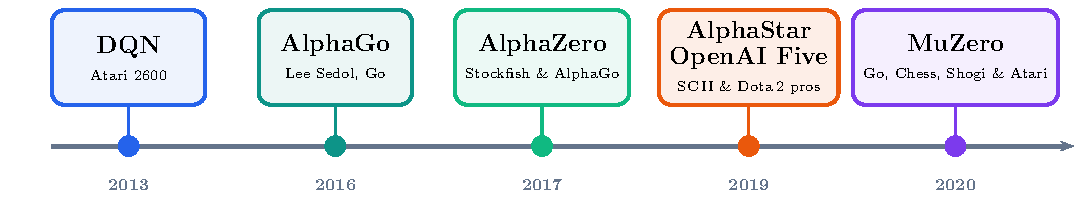
\includegraphics[width=\linewidth]{chapters/05_deep_rl_approaches_rts/figures/drl_timeline.pdf}
    % \caption{Major deep reinforcement learning milestones in strategic games ($2013$--$2020$).}
    \caption[Major DRL milestones in strategic games]{Selected major DRL milestones in strategic games ($2013$--$2020$); not exhaustive.}
    \label{fig:drl-timeline}
\end{figure}

\vspace{-1em}

\subsection{Foundational Breakthroughs in Turn-Based Games}

DQN ($2013$) proved that convolutional neural networks (CNN) could learn control policies from raw pixels on Atari games~\cite{mnihHumanlevelControlDeep2015}. AlphaGo~\cite{silverMasteringGameGo2016} ($2016$) used supervised learning (SL) on human games to initialize a policy network, refined it through RL self-play, and combined it with MCTS to defeat world champion Lee Sedol in Go. AlphaZero~\cite{silverMasteringChessShogi2017} ($2017$) generalized this to Go, Chess, and Shogi through pure self-play without human knowledge. MuZero~\cite{schrittwieserMasteringAtariGo2020} ($2020$) extended this to the model-based setting by learning a latent dynamics model without access to game rules, matching AlphaZero's performance while also mastering Atari.

These systems marked major milestones for AI in strategic games. However, compared with RTS games, these environments remain simpler along several dimensions: board games are turn-based and fully observable, while Atari involves a single agent with a much smaller action space and no simultaneous multi-unit control.

\subsection{Scaling DRL to RTS Games}

The transition from turn-based environments to real-time multi-agent games came with AlphaStar~\cite{vinyalsGrandmasterLevelStarCraft2019} ($2019$), which reached Grandmaster level in StarCraft~II by combining SL from human replays with RL through competitive league training. Concurrently, OpenAI Five~\cite{openaiDota2Large2019} defeated Dota~2 world champions using PPO with pure self-play. Both systems required massive computational resources: OpenAI Five trained on $256$ GPUs and $128\,000$ central processing unit (CPU) cores for $10$ months.

Subsequent work focused on reducing this computational cost. StarCraft Commander (SCC)~\cite{wangSCCEfficientDeep2020} matched StarCraft~II performance with an order of magnitude less computation, while AlphaStar Unplugged~\cite{mathieuAlphaStarUnpluggedLargeScale2023} trained competitive agents entirely from offline replay data.

\section{DRL at Full RTS Scale: AlphaStar}
\label{sec:alphastar}

AlphaStar~\cite{vinyalsGrandmasterLevelStarCraft2019} reached StarCraft~II Grandmaster level (top $0.15$\% of human players) in $2019$, the first AI system to achieve professional-level play in a full-scale RTS environment. Training required $384$ TPUs and $1\,800$ CPUs across the training league over $44$ days, with each agent accumulating $200$ years of simulated game time. This scale is not reproducible in an academic setting. Nevertheless, several of AlphaStar's design choices transfer to smaller environments and have directly influenced the present design (Chapters~\ref{chap:architectures} and~\ref{chap:training-system}); Figure~\ref{fig:alphastar-architecture} gives a high-level overview.

\begin{figure}[!ht]
    \centering
    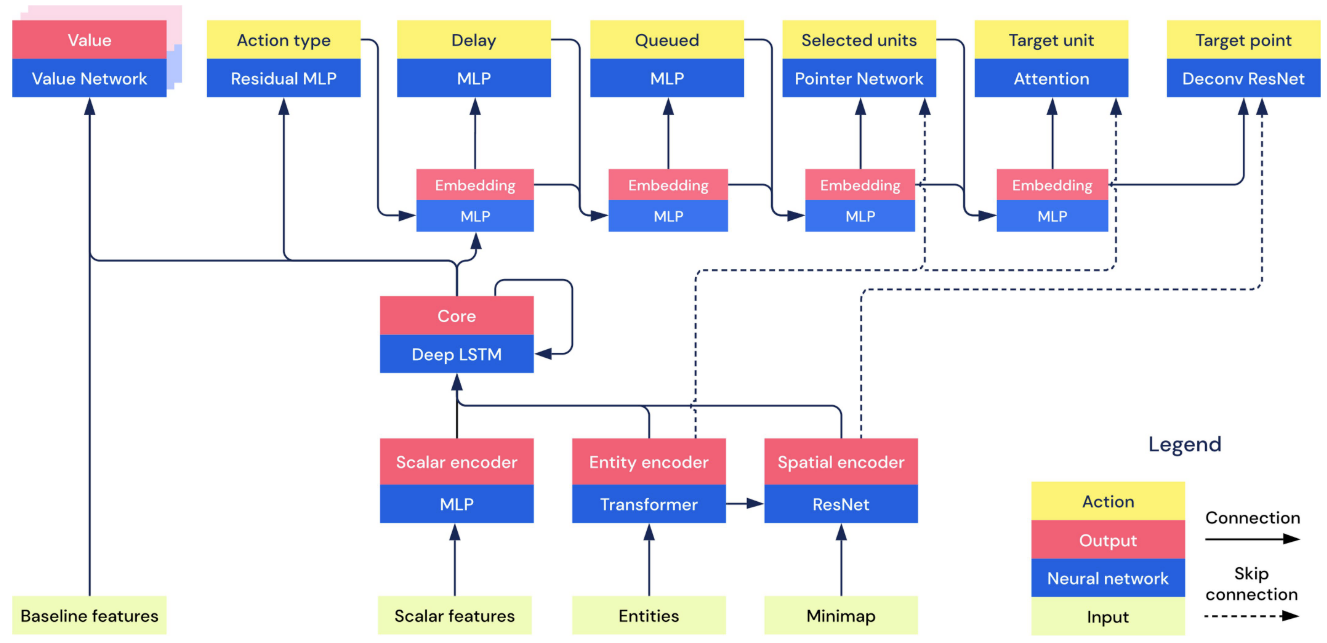
\includegraphics[width=\linewidth]{chapters/05_deep_rl_approaches_rts/figures/nature-alphastar-model.png}
    \caption[AlphaStar architecture]{AlphaStar architecture from~\cite{vinyalsGrandmasterLevelStarCraft2019}. Three input streams (Scalar features, Entities, Minimap) are processed by a Multilayer Perceptron (MLP), a Transformer, and a Residual Network (ResNet) respectively; the Entity and Spatial encoders are linked through a scatter connection to combine spatial and non-spatial features. The encoded representations feed the core deep Long Short-Term Memory (LSTM)~\cite{hochreiterLongShortTermMemory1997}, whose output drives six auto-regressive action heads (Action type, Delay, Queued, Selected units, Target unit, Target point) connected through Embedding/MLP modules. Each head uses a specialized output mechanism (Residual MLP, MLP, MLP, Pointer Network~\cite{vinyalsPointerNetworks2015}, Attention, Deconvolutional ResNet). Dashed skip connections route encoder representations directly to the pointer, attention, and deconvolutional heads. A separate Value Network combines the LSTM output with privileged baseline features (training-only state information not accessible to the policy, e.g. the opponent's hidden units) to produce the critic estimate $\hat{V}(s_t)$.}
    \label{fig:alphastar-architecture}
\end{figure}

\vspace{-1.5em}

\subsection{Observation Encoding}

Two of AlphaStar's encoding choices respond to fog-of-war: a deep LSTM that aggregates information across time, and privileged opponent features fed to the Value Network during training. Training in the fully observable MicroRTS setting removes one of the main motivations for recurrent memory and privileged critic inputs, although recurrence could still help capture temporal patterns such as opponent strategies or production histories. This thesis therefore opts for a simpler frame-stacking approach (Chapter~\ref{chap:training-system}), with the actor and critic sharing the same observation. What does transfer is the entity-spatial representation pair linked through scatter connections: a Transformer over per-unit features fused with a CNN over the map. The same fusion, well-suited to the heterogeneous unit composition typical of RTS games, is adopted in Chapter~\ref{chap:architectures}.

\subsection{Action Space}

StarCraft~II's ${\sim}10^{26}$-action space forces AlphaStar to sample one action per step through six conditional heads, paying an auto-regressive cost at every decision. MicroRTS factorizes along a different axis: GridNet~\cite{huangGym$m$RTSAffordableFull2021} predicts all per-cell actions in a single forward pass under conditional independence (Chapter~\ref{chap:architectures}), which is much cheaper but cannot model dependencies between simultaneous unit decisions. To recover some expressiveness within each unit's factored action, an optional auto-regressive sub-action head inspired by AlphaStar is implemented (Chapter~\ref{chap:training-system}).

\subsection{Training Pipeline}

AlphaStar's training has two phases: SL on ${\sim}970\,000$ human replays produces a Diamond-level initialization, then RL refines the policy through league self-play, using V-trace~\cite{espeholtIMPALAScalableDistributed2018} for off-policy correction, upgoing policy update (UPGO) for self-imitation, and TD($\lambda$) for value learning. The supervised warmstart is retained directly, with bot replays substituting for the unavailable human dataset (evaluated in Chapter~\ref{chap:results}). AlphaStar's \emph{pseudo-rewards} steer the agent toward human strategies: at the start of each episode, a target statistic $z$ (build order, unit composition) is sampled from a database of human replays, and the agent receives auxiliary rewards throughout the episode proportional to how closely its behavior matches $z$. This thesis instead uses \emph{reward scheduling}, which progressively anneals dense hand-crafted shaping signals (resource gathering, unit production) toward the sparse terminal win/loss reward over training (Chapter~\ref{chap:training-system}). The two mechanisms address the same problem (sparse-reward learning) but in opposite directions: AlphaStar adds a dense signal to imitate known human strategies, whereas reward scheduling removes the dense signal so the agent eventually optimizes the true game outcome alone. The off-policy machinery (V-trace, UPGO) is also dropped, since vanilla PPO suffices at MicroRTS scale and avoids the engineering overhead.

\subsection{League Training and PFSP}

Na\"ive self-play suffers from \emph{strategy cycling}: an agent learns strategy A that beats B, then B that beats A, forgetting earlier solutions in a non-transitive loop. AlphaStar's league of concurrent agents addresses this through three role types. \emph{Main agents} train against the entire population via Prioritized Fictitious Self-Play (PFSP), sampling opponent $i$ with probability proportional to $(1 - \mathrm{WR}_i)^p$ so harder opponents are seen more often\footnote{The exponent $p \geq 1$ controls how sharply sampling concentrates on the hardest opponents: at $p = 1$, weights are linear in $1 - \mathrm{WR}_i$, while larger $p$ amplifies the gap. AlphaStar~\cite{vinyalsGrandmasterLevelStarCraft2019} uses $p = 2$ in its \emph{hard} PFSP variant.}. Two auxiliary populations of \emph{exploiters} probe weaknesses and are periodically reset to keep exploration fresh, while frozen checkpoints accumulate to prevent catastrophic forgetting of counter-strategies. This thesis implements the same PFSP weighting and checkpoint pool (Chapter~\ref{chap:training-system}); the exploiter populations are omitted as the training budget does not justify the parallel agents.

\section{DRL at MicroRTS Scale}
\label{sec:microRTS_sota}

Attention now turns to MicroRTS, the environment at the center of this thesis. Despite being actively maintained since $2013$ and hosting annual competitions since $2017$, the DRL literature on MicroRTS remains sparse~\cite{barrosesaDeepReinforcementLearning2025, endlaDeepReinforcementLearning2025}: only a handful of studies exist, most competition entries remain rule-based, search-based, or hybrid (Chapter~\ref{chap:historical-approach}), and RAISocketAI remains the only DRL agent to have won the competition. This scarcity is a primary motivation for the present thesis.

\vspace{-0.2em}

\subsection{Early Exploration ($2019$--$2020$)}
Two foundational studies established the basic learning paradigm. Huang et al.~\cite{huangComparingObservationAction2019} compared global and local representations for both observations and actions: the global setting treats the game as a single decision-maker selecting one action per step, while the local setting decentralizes control by letting each unit independently select its action conditioned on local context. On resource gathering tasks, the local setting consistently outperformed the global one, motivating the per-cell action factorization that GridNet would later formalize (with a centralized observation and a single shared policy). Kelly and Churchill~\cite{kellyTransferLearningRTS} reported that value-based methods (DQN variants~\cite{vanhasseltDeepReinforcementLearning2015, wangDuelingNetworkArchitectures2015}) struggled with the combinatorial joint action space of RTS domains, while policy-gradient methods showed more promise. These studies established two design principles adopted by the field: spatial action factorization and policy-gradient training.

\vspace{-0.2em}

\subsection{Gym-$\mu$RTS and GridNet ($2020$--$2021$)}
The release of Gym-$\mu$RTS~\cite{huangGym$m$RTSAffordableFull2021} provided Gymnasium-compatible interfaces with factorized action spaces, invalid action masking~\cite{huangCloserLookInvalid2022}, and vectorized environments (Chapter~\ref{chap:python_bridge}). The paper also popularizes \urlref{https://github.com/Farama-Foundation/MicroRTS-Py}{\textbf{GridNet}}, the standard architectural pattern for MicroRTS: a fully convolutional encoder-decoder predicting one action per grid cell in parallel under a conditional independence assumption. A PPO agent trained with GridNet for ${\sim}60$ hours achieved ${\sim}89$\% $\mathrm{WR}$ on the standard \emph{basesWorkers16x16A} map against the $2021$-era scripted opponent pool, one of the first DRL systems to become competitive against classical MicroRTS bots. However, training was limited to a single map and the agent was only evaluated as Player~$0$ (P0) from a fixed starting position.

\vspace{-0.2em}

\subsection{RAISocketAI ($2023$--$2024$)}
\urlref{https://github.com/sgoodfriend/rl-algo-impls/tree/main/rl_algo_impls/microrts}{RAISocketAI}~\cite{goodfriendCompetitionWinningDeep2024} became the first DRL agent to win the MicroRTS competition (IEEE CoG $2023$), achieving ${\sim}72$\% $\mathrm{WR}$ across all matchups. The system uses a \emph{DoubleCone} (4, 6, 4) architecture, adapted from the fourth-place Lux AI Season 2 model: $4$ full-resolution residual blocks, an encoder-decoder block downsampling by stride $4$ to process $6$ residual blocks at quarter resolution before upsampling (with a residual skip across the down-up section), and $4$ final full-resolution blocks, each block equipped with Squeeze-and-Excitation (SE) channel attention. Since DoubleCone exceeds the $100$~ms per-turn budget on larger maps, RAISocketAI also includes \emph{squnet}, a U-Net variant with more aggressive downscaling that requires up to $8\times$ fewer operations on $64{\times}64$ maps.

PPO training, alternating between self-play and scripted opponents in a curriculum, annealing shaped rewards (resource gathering, unit production) toward sparse terminal ones during training. At inference, RAISocketAI deploys a \emph{portfolio} of up to seven specialized models selected by map size, with map-specific fine-tuning on three maps that diverge most from the training distribution.

The paper also reports a BC-PPO variant that combines behavior cloning (BC) pre-training on bot replays~\cite{ontanonExperimentsLearningUnitAction2016} with PPO fine-tuning, achieving ${\sim}88$\% in benchmark round-robin\footnote{Single-player round-robin against WorkerRush, LightRush, CoacAI, and Mayari on the eight open maps (Chapter~\ref{chap:evaluation-framework}).} without map-specific fine-tuning, suggesting that imitation warmstarts improve cross-map generalization. Total compute for the full portfolio reached ${\sim}1.5$ billion environment steps and ${\sim}70$ GPU-days, encompassing base self-play training, iterative fine-tuning against CoacAI/Mayari, transfer learning to map-specific models on the three larger Open maps, and the alternative squnet models for larger maps. Of this total, ${\sim}23.6$ GPU-days were spent solely on the $16{\times}16$ DoubleCone model. The follow-up BC-PPO variant required an additional ${\sim}72$ GPU-days (${\sim}23$ for behavior cloning, ${\sim}49$ for PPO fine-tuning).

\vspace{-0.2em}

\subsection{Recent Directions ($2024$--$2025$)}

Reinforcement Learning as a Rehearsal (RLaR)~\cite{manandharReinforcementActorcriticLearning2024} couples actor-critic RL with an auxiliary prediction function exploiting privileged information available at training to guide exploration under partial observability. Lemos et al.~\cite{lemosEnhancingDeepReinforcement2025} address a generalization bottleneck of GridNet, namely the critic's reliance on a fixed-size flatten before its dense layers. They integrate a Spatial Pyramid Pooling (SPP) layer into the critic, producing a fixed-length representation regardless of map size and enabling a single agent to play maps of arbitrary dimensions. This thesis adopts both directions in its training system (Chapter~\ref{chap:training-system}): an auxiliary opponent-modeling head predicts the opponent's next action to bias the encoder toward strategically informative features, and an SPP-equipped critic decouples the network from a fixed map resolution.

\vspace*{-0.2cm}

\section{Thesis Contributions}
\label{sec:thesis_positioning}

\vspace*{-0.1cm}

This thesis builds on Gym-$\mu$RTS~\cite{huangGym$m$RTSAffordableFull2021} and draws design inspiration from RAISocketAI~\cite{goodfriendCompetitionWinningDeep2024} and AlphaStar~\cite{vinyalsGrandmasterLevelStarCraft2019}. Six contributions address the gaps surveyed above (sparse DRL literature on MicroRTS, limited Gym-$\mu$RTS pipeline, no systematic ablations, $2026$ CoG shift to LLM-based agents).

\paragraph*{1. Reproducible MicroRTS tournament framework (Chapter~\ref{chap:evaluation-framework}).} A self-contained tournament framework, anchored on the $2023$ MicroRTS competition, runs on $12$ maps ($8$ open + $4$ closed), $15$ benchmark agents spanning seven competition editions, and four game-theoretic metrics (Nash averaging, $\alpha$-Rank, Copeland, worst-case and average regret).

\vspace*{-0.04cm}

\paragraph*{2. Extended and modular Java-Python bridge (Chapter~\ref{chap:python_bridge}).} The Gym-$\mu$RTS bridge is extended with self-play, multi-map padding, filtered action masking, symmetry augmentation, composable observation and action wrappers, and a reserved-observation channel, all opt-in and preserving numerical equivalence with the baseline.

\vspace*{-0.04cm}

\paragraph*{3. UECD architecture and incremental design path (Chapters~\ref{chap:architectures} and~\ref{chap:results}).} \code{UECD}, one of the first MicroRTS architectures with explicit per-unit Transformer reasoning, integrates a CBAM-gated U-Net (local spatial), an Entity Transformer (unit-to-unit), and bottleneck self-attention (global spatial) into a single policy. Seven intermediate architectures from GridNet to \code{UECD} trace the design path, each ablated across three seeds.

\vspace*{-0.04cm}

\paragraph*{4. Modular training pipeline with systematic ablations (Chapters~\ref{chap:training-system} and~\ref{chap:results}).} Flag-gated PPO mechanisms span five axes (action sampling, reward and value signal, opponent curriculum and self-play, auxiliary representation, generalization and architecture). Each is ablated across three seeds, driving the final recipe.

\vspace*{-0.04cm}

\paragraph*{5. An analysis of discount-induced reward collapse (Chapter~\ref{chap:results}).} A formal derivation explains a training instability arising when the shaped reward is annealed to zero: once only the terminal reward survives, the empirical PPO advantage favors shorter episodes by $\gamma^{-\Delta}$, driving the policy into a degenerate rush that wins against the training pool but collapses against held-out opponents. The analysis isolates the three causal conditions and the mitigations that break them, a result transferable to any shaped-to-sparse reward annealing schedule.

\vspace*{-0.04cm}

\paragraph*{6. Compute-efficient single-map champion (Chapter~\ref{chap:results}).} \code{UECD-Best}, combining \code{UECD} with the top features and a two-phase opponent-pool fine-tuning schedule, reaches a \textbf{96.67\%} overall win rate on the standard \emph{basesWorkers16x16A} map in a $19$-agent tournament, ranking first on three of four game-theoretic metrics. Against RAISocketAI, it holds a \textbf{65.7\%} head-to-head win rate (stochastic $1\,000$-game protocol) at \textbf{9.47} GPU-days of training.

\vspace*{0.1cm}
A paper distilling the contributions and results of this thesis has been submitted to IEEE CoG 2026
(currently under review).